% ============================================================
%  chapter12_slides.tex
%  Beamer slides — Chapter 12: Linear Programming
%  Algorithms for Optimization, 2nd ed. (2026)
%  Kochenderfer & Wheeler
% ============================================================
\documentclass[aspectratio=169,10pt]{beamer}

\usetheme{Madrid}
\usecolortheme{seahorse}

\usepackage[T1]{fontenc}
\usepackage[utf8]{inputenc}
\usepackage{amsmath,amssymb,amsfonts}
\usepackage{mathtools}
\usepackage{bm}
\usepackage{graphicx}
\usepackage{booktabs}
\usepackage{array}
\usepackage{colortbl}
\usepackage{xcolor}
\usepackage{listings}
\usepackage{tikz}
\usepackage{pgfplots}
\pgfplotsset{compat=1.18}
\usetikzlibrary{arrows.meta,positioning,shapes,calc}
\usepackage{multicol}

\graphicspath{{figures/}}

% -- Listings style (Python) --------------------------------------------------
\definecolor{codebg}{rgb}{0.97,0.97,0.97}
\definecolor{codeframe}{rgb}{0.7,0.7,0.7}
\definecolor{kwcolor}{rgb}{0.0,0.4,0.7}
\definecolor{strcolor}{rgb}{0.6,0.1,0.1}
\definecolor{cmtcolor}{rgb}{0.3,0.5,0.3}

\lstset{
  language=Python,
  basicstyle=\ttfamily\scriptsize,
  keywordstyle=\color{kwcolor}\bfseries,
  stringstyle=\color{strcolor},
  commentstyle=\color{cmtcolor}\itshape,
  numbers=left,
  numberstyle=\tiny\color{gray},
  stepnumber=1,
  frame=single,
  backgroundcolor=\color{codebg},
  breaklines=true,
  showstringspaces=false,
  tabsize=4,
  extendedchars=false,
  keepspaces=true,
}

% -- Beamer settings -----------------------------------------------------------
\setbeamertemplate{footline}[frame number]
\setbeamertemplate{navigation symbols}{}
\setbeamerfont{footnote}{size=\tiny}

% -- Math operators -----------------------------------------------------------
\DeclareMathOperator*{\minimize}{minimize}
\DeclareMathOperator*{\maximize}{maximize}
\newcommand{\subjectto}{\text{subject to}}

% -- Convenience macros -------------------------------------------------------
\newcommand{\Rn}{\mathbb{R}^n}
\newcommand{\xv}{\mathbf{x}}
\newcommand{\cv}{\mathbf{c}}
\newcommand{\bv}{\mathbf{b}}
\newcommand{\Av}{\mathbf{A}}
\newcommand{\wv}{\mathbf{w}}
\newcommand{\sv}{\mathbf{s}}
\newcommand{\zv}{\mathbf{z}}
\newcommand{\muv}{\boldsymbol{\mu}}
\newcommand{\lav}{\boldsymbol{\lambda}}
\newcommand{\calB}{\mathcal{B}}
\newcommand{\calV}{\mathcal{V}}

% -- Title info ----------------------------------------------------------------
\title[Chapter 12: Linear Programming]{Chapter 12: Linear Programming}
\subtitle{Algorithms for Optimization, 2\textsuperscript{nd} ed.\ (2026)}
\author{Kochenderfer \& Wheeler}
\date{2026}

% -----------------------------------------------------------------------------
\begin{document}
% -----------------------------------------------------------------------------

\begin{frame}
  \titlepage
\end{frame}

% -----------------------------------------------------------------------------
\begin{frame}{Table of Contents}
  \tableofcontents
\end{frame}

% -----------------------------------------------------------------------------
\section{Introduction}
% -----------------------------------------------------------------------------

\begin{frame}{What is Linear Programming?}
  \begin{columns}
    \begin{column}{0.58\textwidth}
      \begin{block}{Definition}
        A \textbf{linear program (LP)} consists of a \emph{linear objective function}
        and a set of \emph{linear constraints}:
        \[
          \minimize_{\xv}\; \cv^\top\xv \quad
          \text{subject to linear equalities/inequalities in }\xv
        \]
      \end{block}
      \vspace{4pt}
      \textbf{Applications:}
      \begin{itemize}
        \item Transportation \& logistics
        \item Communication networks
        \item Manufacturing, economics
        \item Operations research
        \item $L_1$ / $L_\infty$ regression (converted to LP)
      \end{itemize}
    \end{column}
    \begin{column}{0.40\textwidth}
      \begin{block}{Key Properties}
        \begin{itemize}
          \item Linear objective $\Rightarrow$ flat ``ramp''
          \item Feasible set is a \emph{convex polytope}
          \item Any local minimum is a \emph{global} minimum
          \item Modern solvers: millions of variables \& constraints
        \end{itemize}
      \end{block}
      \vspace{4pt}
      \centering
      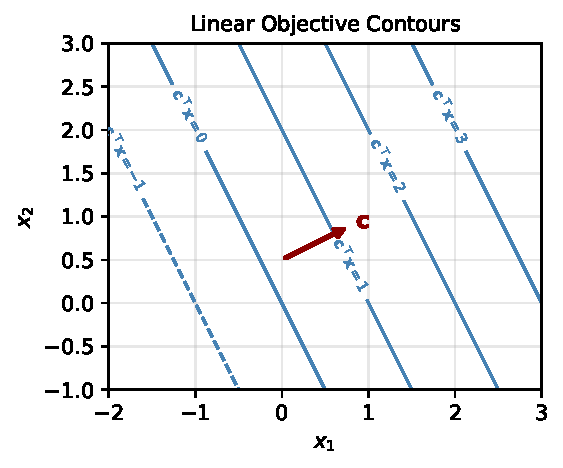
\includegraphics[width=0.85\textwidth]{linear_contours.pdf}
      \vspace{-4pt}
      {\tiny Contours of $\cv^\top\xv$; increase in direction $\cv$}
    \end{column}
  \end{columns}
\end{frame}

% -----------------------------------------------------------------------------
\section{Problem Formulation}
% -----------------------------------------------------------------------------

\begin{frame}{12.1 Problem Formulation --- General Form}
  \begin{block}{General Form (Eq.\ 12.2)}
    \[
      \minimize_{\xv}\;\cv^\top\xv
      \quad\text{subject to}\quad
      \Av_{\mathrm{LE}}\,\xv \le \bv_{\mathrm{LE}},\quad
      \Av_{\mathrm{EQ}}\,\xv = \bv_{\mathrm{EQ}}
    \]
    \begin{itemize}
      \item $\cv, \xv \in \mathbb{R}^n$ --- cost vector and design variables
      \item $\Av_{\mathrm{LE}} \in \mathbb{R}^{p\times n}$, $\bv_{\mathrm{LE}} \in \mathbb{R}^p$ --- inequality rows
      \item $\Av_{\mathrm{EQ}} \in \mathbb{R}^{q\times n}$, $\bv_{\mathrm{EQ}} \in \mathbb{R}^q$ --- equality rows
    \end{itemize}
  \end{block}

  \vspace{6pt}
  \begin{columns}
    \begin{column}{0.48\textwidth}
      \begin{exampleblock}{Example 12.1 --- Concrete LP}
        \small
        \[
          \minimize_{x_1,x_2,x_3}\;2x_1-3x_2+7x_3
        \]
        \[
          \text{s.t.}\quad
          \begin{aligned}
            2x_1+3x_2-8x_3 &\le 5\\
            4x_1+\phantom{0}x_2+3x_3 &\le 9\\
            x_1-5x_2-3x_3 &\ge -4\\
            x_1+\phantom{0}x_2+2x_3 &= 1
          \end{aligned}
        \]
      \end{exampleblock}
    \end{column}
    \begin{column}{0.48\textwidth}
      \begin{exampleblock}{Example 12.2 --- Norm Minimization as LP}
        \small
        $\minimize\|\Av\xv-\bv\|_1$ is equivalent to:
        \[
          \minimize_{\xv,\sv}\;\mathbf{1}^\top\sv
          \quad\text{s.t.}\quad
          \Av\xv-\bv \le \sv,\;
          \Av\xv-\bv \ge -\sv
        \]
        $\minimize\|\Av\xv-\bv\|_\infty$ $\Leftrightarrow$ minimize scalar $t$\,:
        \[
          \Av\xv-\bv\le t\mathbf{1},\quad \Av\xv-\bv\ge -t\mathbf{1}
        \]
      \end{exampleblock}
    \end{column}
  \end{columns}
\end{frame}

% -----------------------------------------------------------------------------
\begin{frame}{Standard Form}
  \begin{block}{Standard Form (Eq.\ 12.3)}
    \[
      \minimize_{\xv}\;\cv^\top\xv
      \quad\text{subject to}\quad
      \Av\xv \le \bv,\quad \xv \ge \mathbf{0}
    \]
    All constraints are \emph{less-than inequalities}; all variables are \emph{nonnegative}.
  \end{block}

  \vspace{6pt}
  \textbf{Conversion rules:}
  \begin{enumerate}
    \item \textbf{Equality $\to$ two inequalities} (Eq.\ 12.4):
      \[
        \Av_{\mathrm{EQ}}\xv = \bv_{\mathrm{EQ}}
        \;\longrightarrow\;
        \Av_{\mathrm{EQ}}\xv \le \bv_{\mathrm{EQ}},\quad
        -\Av_{\mathrm{EQ}}\xv \le -\bv_{\mathrm{EQ}}
      \]
    \item \textbf{Free variable $\to$ positive/negative split} (Eq.\ 12.6):
      Replace $\xv$ with $\xv^+ - \xv^-$, constrain $\xv^+,\xv^- \ge \mathbf{0}$:
      \[
        \minimize_{\xv^+,\xv^-}
        \begin{bmatrix}\cv^\top & -\cv^\top\end{bmatrix}
        \begin{bmatrix}\xv^+\\\xv^-\end{bmatrix}
        \;\text{s.t.}\;
        \begin{bmatrix}\Av & -\Av\end{bmatrix}
        \begin{bmatrix}\xv^+\\\xv^-\end{bmatrix}
        \le \bv,\;
        \begin{bmatrix}\xv^+\\\xv^-\end{bmatrix}\ge\mathbf{0}
      \]
  \end{enumerate}
\end{frame}

% -----------------------------------------------------------------------------
\begin{frame}{Equality Form and Slack Variables}
  \begin{columns}
    \begin{column}{0.54\textwidth}
      \begin{block}{Equality Form (Eq.\ 12.7)}
        \[
          \minimize_{\xv}\;\cv^\top\xv
          \quad\text{s.t.}\quad
          \Av\xv = \bv,\quad \xv \ge \mathbf{0}
        \]
        \begin{itemize}
          \item $\xv\in\mathbb{R}^n$, $\Av\in\mathbb{R}^{m\times n}$, $\bv\in\mathbb{R}^m$
          \item $m$ equality constraints, $n$ nonneg.\ variables
          \item Preferred form for the simplex algorithm
        \end{itemize}
      \end{block}

      \begin{block}{Standard $\to$ Equality via Slack Variables (Eq.\ 12.8)}
        \[
          \Av\xv \le \bv
          \;\xrightarrow{\text{add }\sv\ge\mathbf{0}}\;
          \Av\xv + \sv = \bv,\quad \sv\ge\mathbf{0}
        \]
        \[
          \minimize_{\xv,\sv}
          \begin{bmatrix}\cv^\top & \mathbf{0}^\top\end{bmatrix}
          \begin{bmatrix}\xv\\\sv\end{bmatrix}
          \;\text{s.t.}\;
          \begin{bmatrix}\Av & \mathbf{I}\end{bmatrix}
          \begin{bmatrix}\xv\\\sv\end{bmatrix}
          =\bv,\;
          \begin{bmatrix}\xv\\\sv\end{bmatrix}\ge\mathbf{0}
        \]
      \end{block}
    \end{column}
    \begin{column}{0.44\textwidth}
      \begin{exampleblock}{Example 12.3 --- Slack Variable Illustration}
        \small
        Standard form: $\minimize_x\; x$ s.t.\ $x\ge 1$

        Equality form (add slack $s\ge0$):
        \[
          \minimize_{x,s}\; x
          \quad\text{s.t.}\quad
          x - s = 1,\;x,s\ge0
        \]
        The equality constraint restricts feasible points to the line $x-s=1$.
      \end{exampleblock}
      \centering
      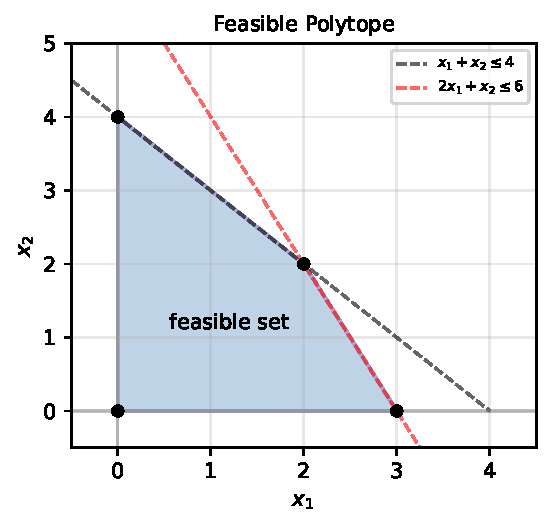
\includegraphics[width=0.85\textwidth]{feasible_polytope.pdf}
      {\tiny Feasible polytope: intersection of linear constraints}
    \end{column}
  \end{columns}
\end{frame}

% -----------------------------------------------------------------------------
\begin{frame}{Geometric Interpretation}
  \begin{columns}
    \begin{column}{0.46\textwidth}
      \textbf{Half-space:}
      \begin{itemize}
        \item Constraint $\wv^\top\xv \le b$ defines a \emph{half-space}
        \item Hyperplane $\wv^\top\xv=b$ is perpendicular to $\wv$
        \item Region $\wv^\top\xv>b$ is on the $+\wv$ side
        \item Region $\wv^\top\xv<b$ is on the $-\wv$ side
      \end{itemize}
      \vspace{4pt}
      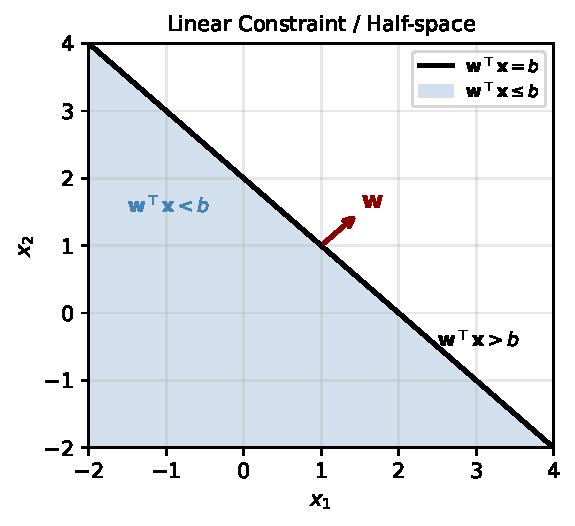
\includegraphics[width=\textwidth]{halfspace.pdf}
    \end{column}
    \begin{column}{0.52\textwidth}
      \textbf{Four outcome types (Figure 12.4):}
      \vspace{4pt}
      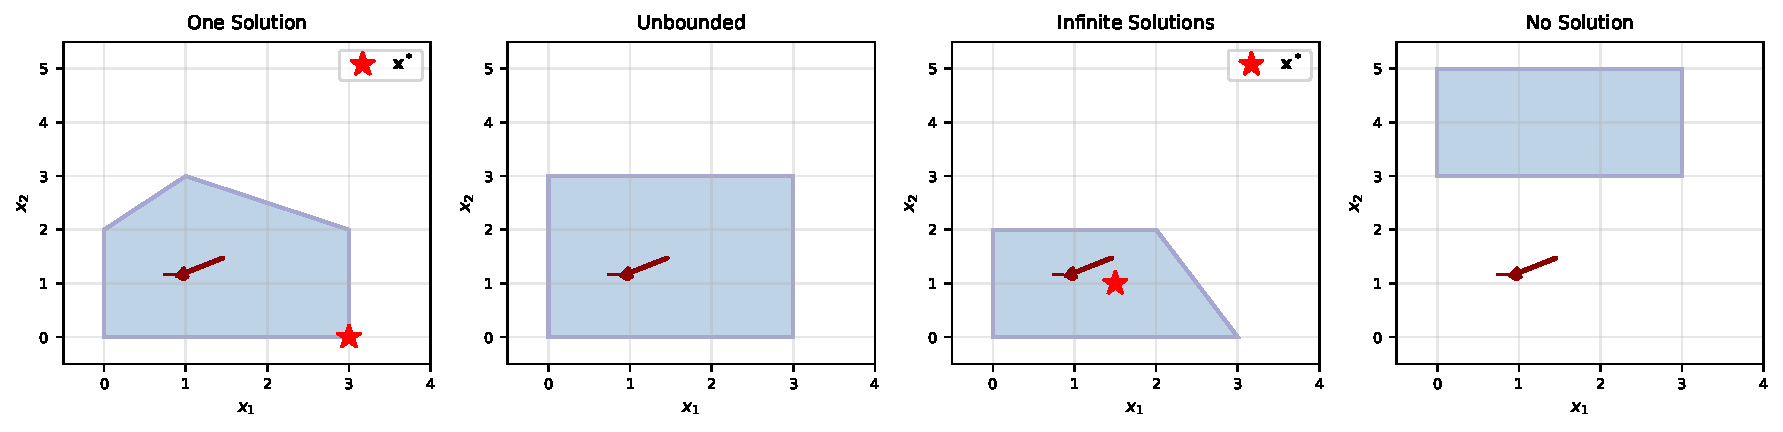
\includegraphics[width=\textwidth]{lp_cases.pdf}
      \vspace{4pt}
      \begin{itemize}
        \item \textbf{One solution}: optimal at a vertex
        \item \textbf{Unbounded}: feasible set extends to $-\infty$
        \item \textbf{Infinite solutions}: optimal face $\perp\cv$
        \item \textbf{No solution}: over-constrained, infeasible
      \end{itemize}
    \end{column}
  \end{columns}
\end{frame}

% -----------------------------------------------------------------------------
\begin{frame}{Example 12.4 --- Standard to Equality Form}
  \begin{exampleblock}{Conversion: maximize $5x_1+4x_2$ subject to $2x_1+3x_2\le5$, $4x_1+x_2\le11$}
    \textbf{Step 1}: Convert to minimization (negate objective):
    \[
      \minimize_{x_1,x_2}\;-5x_1-4x_2
    \]
    \textbf{Step 2}: Introduce slack variables $s_1,s_2\ge0$:
    \[
      \begin{aligned}
        2x_1+3x_2+s_1 &= 5\\
        4x_1+\phantom{3}x_2+s_2 &= 11
      \end{aligned}
    \]
    \textbf{Step 3}: Split free variables $x_1,x_2$ into $x_i^+,x_i^-\ge0$:
    \[
      \minimize_{x_1^+,x_1^-,x_2^+,x_2^-,s_1,s_2}
      -5(x_1^+-x_1^-)-4(x_2^+-x_2^-)
    \]
    \[
      \text{s.t.}\quad
      2(x_1^+-x_1^-)+3(x_2^+-x_2^-)+s_1=5,\quad
      4(x_1^+-x_1^-)+(x_2^+-x_2^-)+s_2=11
    \]
    \[
      x_1^+,x_1^-,x_2^+,x_2^-,s_1,s_2\ge0
    \]
  \end{exampleblock}
  \centering
  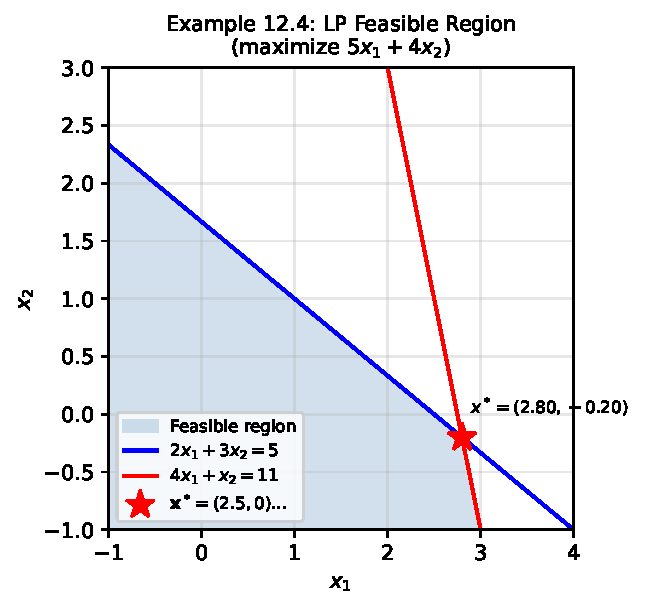
\includegraphics[width=0.35\textwidth]{example124.pdf}
\end{frame}

% -----------------------------------------------------------------------------
\begin{frame}[fragile]{Python: Building LP Standard/Equality Form}
\begin{lstlisting}
import numpy as np
from scipy.optimize import linprog

# -- Example 12.1 via scipy linprog ------------------------------------------
# minimize  2x1 - 3x2 + 7x3
# s.t.      2x1 + 3x2 - 8x3 <=  5
#           4x1 +  x2 + 3x3 <=  9
#          -x1 + 5x2 + 3x3  <=  4    (flipped from x1-5x2-3x3 >= -4)
#           x1 +  x2 + 2x3  ==  1    (equality)

c      = np.array([ 2.0, -3.0,  7.0])
A_ub   = np.array([[ 2,  3, -8],
                   [ 4,  1,  3],
                   [-1,  5,  3]])
b_ub   = np.array([5.0, 9.0, 4.0])
A_eq   = np.array([[1, 1, 2]])
b_eq   = np.array([1.0])

res = linprog(c, A_ub=A_ub, b_ub=b_ub,
              A_eq=A_eq, b_eq=b_eq, method='highs')
print("Optimal x :", res.x)
print("Optimal f :", res.fun)

# -- L1 minimization as LP (Example 12.2) ------------------------------------
def l1_min_lp(A, b):
    """Minimize ||Ax - b||_1  via LP."""
    m, n = A.shape
    # variables: [x (n), s (m)]
    c_lp = np.concatenate([np.zeros(n), np.ones(m)])
    # Ax - b <= s  =>  [A, -I][x;s] <= b
    A_ub_l1 = np.hstack([ A, -np.eye(m)])
    # -(Ax-b) <= s => [-A, -I][x;s] <= -b
    A_ub_l2 = np.hstack([-A, -np.eye(m)])
    A_ub_combined = np.vstack([A_ub_l1, A_ub_l2])
    b_ub_combined = np.concatenate([b, -b])
    return linprog(c_lp, A_ub=A_ub_combined, b_ub=b_ub_combined)
\end{lstlisting}
\end{frame}

% -----------------------------------------------------------------------------
\section{Simplex Algorithm}
% -----------------------------------------------------------------------------

\begin{frame}{12.2 Simplex Algorithm --- Overview}
  \begin{columns}
    \begin{column}{0.50\textwidth}
      \begin{block}{Core Idea}
        Move from \textbf{vertex to vertex} of the feasible polytope,
        decreasing the objective at each step, until optimality is confirmed.
      \end{block}
      \vspace{6pt}
      \textbf{Two phases:}
      \begin{enumerate}
        \item \textbf{Initialization phase}: Find an initial feasible vertex
          (by solving an auxiliary LP)
        \item \textbf{Optimization phase}: Traverse adjacent vertices
          following the steepest descent direction
      \end{enumerate}
      \vspace{6pt}
      \begin{alertblock}{Requirements for the Simplex Method}
        \begin{itemize}
          \item LP must be in \textbf{equality form}: $\Av\xv=\bv$, $\xv\ge\mathbf{0}$
          \item Rows of $\Av$ must be \textbf{linearly independent}
          \item Number of constraints $m \le n$ (not over-constrained)
        \end{itemize}
      \end{alertblock}
    \end{column}
    \begin{column}{0.48\textwidth}
      \centering
      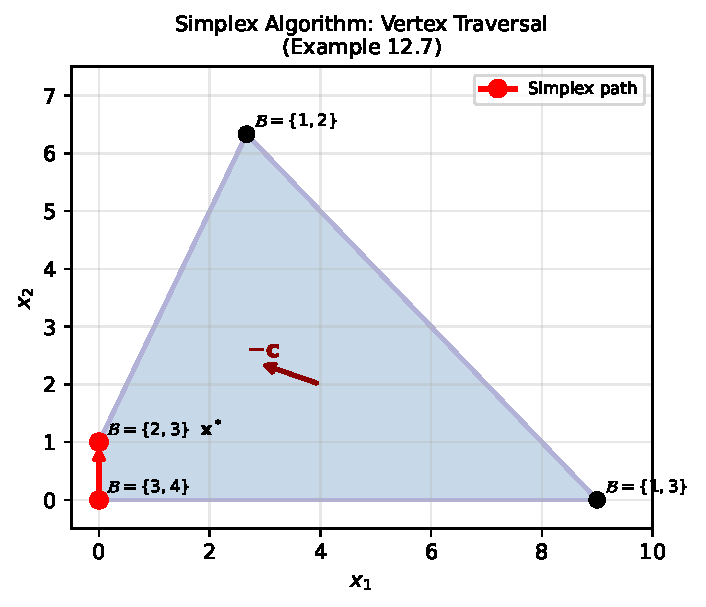
\includegraphics[width=\textwidth]{simplex_traversal.pdf}
      {\small Simplex path on feasible polytope (Example 12.7):\\
       $\calB=\{3,4\} \to \calB=\{2,3\}$ (optimal)}
    \end{column}
  \end{columns}
\end{frame}

% -----------------------------------------------------------------------------
\begin{frame}{12.2.1 Vertices and Partitions}
  \begin{block}{Vertex Characterization}
    Every vertex of the feasible polytope $\{\xv : \Av\xv=\bv,\,\xv\ge\mathbf{0}\}$
    is uniquely defined by setting exactly $n-m$ components of $\xv$ to zero.

    The remaining $n$ indices are partitioned into:
    \[
      \calB \;\cup\; \calV = \{1,\ldots,n\},\quad |\calB|=m,\;|\calV|=n-m
    \]
    \begin{itemize}
      \item $\calB$ (``busy'' / basic): \quad $i\in\calB \Rightarrow x_i \ge 0$ (Eq.\ 12.12)
      \item $\calV$ (``vacant'' / non-basic): $i\in\calV \Rightarrow x_i = 0$ (Eq.\ 12.11)
    \end{itemize}
  \end{block}

  \begin{columns}
    \begin{column}{0.56\textwidth}
      \begin{block}{Extracting a Vertex (Eq.\ 12.13) --- Algorithm 12.1}
        The $m\times m$ submatrix $\Av_\calB$ formed by the $m$ columns of $\Av$
        indexed by $\calB$ must be \emph{invertible}:
        \[
          \Av\xv = \Av_\calB\,\xv_\calB = \bv
          \quad\Rightarrow\quad
          \xv_\calB = \Av_\calB^{-1}\bv
        \]
        If $\Av_\calB$ is invertible, $(\calB,\calV)$ defines a vertex; otherwise not.
      \end{block}
    \end{column}
    \begin{column}{0.42\textwidth}
      \begin{exampleblock}{Example 12.6 --- Verify a Vertex}
        \footnotesize
        $\Av = \begin{bmatrix}1&1&1&1\\0&-1&2&3\\2&1&2&-1\end{bmatrix}$,
        $\xv=[1,1,0,0]$

        Try $\calB=\{1,2,3\}$:
        $\Av_{\{1,2,3\}}$ is invertible $\checkmark$

        Try $\calB=\{1,2,4\}$:
        $\Av_{\{1,2,4\}}$ is invertible $\checkmark$

        $\Rightarrow$ $\xv=[1,1,0,0]$ is a vertex.
      \end{exampleblock}
    \end{column}
  \end{columns}
\end{frame}

% -----------------------------------------------------------------------------
\begin{frame}{12.2.2 First-Order Necessary Conditions (KKT)}
  \begin{block}{Lagrangian for Equality-Form LP (Eq.\ 12.14)}
    \[
      \mathcal{L}(\xv,\muv,\lav)
      = \cv^\top\xv - \muv^\top\xv - \lav^\top(\Av\xv-\bv)
    \]
    Four necessary (and sufficient for LPs) KKT conditions:
    \begin{enumerate}
      \item \textbf{Feasibility}: $\Av\xv=\bv$, $\xv\ge\mathbf{0}$
      \item \textbf{Dual feasibility}: $\muv\ge\mathbf{0}$
      \item \textbf{Complementary slackness}: $\muv\odot\xv=\mathbf{0}$
      \item \textbf{Stationarity}: $\Av^\top\lav + \muv = \cv$
    \end{enumerate}
  \end{block}

  \begin{columns}
    \begin{column}{0.52\textwidth}
      \textbf{Computing $\lav$ and $\muv_\calV$ at a vertex:}

      Set $\muv_\calB=\mathbf{0}$ (complementary slackness with $\xv_\calB\ge\mathbf{0}$):
      \[
        \Av_\calB^\top\lav = \cv_\calB
        \quad\Rightarrow\quad
        \lav = \Av_\calB^{-\top}\cv_\calB \tag{12.17}
      \]
      Then (Eq.\ 12.20):
      \[
        \muv_\calV = \cv_\calV - \bigl(\Av_\calB^{-1}\Av_\calV\bigr)^\top\cv_\calB
      \]
    \end{column}
    \begin{column}{0.46\textwidth}
      \begin{alertblock}{Optimality Test}
        \begin{itemize}
          \item If $\muv_\calV \ge \mathbf{0}$: \textbf{current vertex is optimal}
          \item If any $(\muv_\calV)_q < 0$: vertex is suboptimal;\\
                pivot on index $q$
        \end{itemize}
      \end{alertblock}
    \end{column}
  \end{columns}
\end{frame}

% -----------------------------------------------------------------------------
\begin{frame}{12.2.3 Optimization Phase --- Pivoting}
  \begin{columns}
    \begin{column}{0.54\textwidth}
      \begin{block}{Edge Transition (Eq.\ 12.21--12.24)}
        Choose \textbf{entering index} $q\in\calV$ (with $(\muv_\calV)_q<0$).
        New vertex must satisfy $\Av\xv'=\bv$:
        \[
          \xv'_\calB = \xv_\calB - \Av_\calB^{-1}\Av_{\{q\}}\,x'_q
        \]
        \textbf{Minimum ratio test} --- choose \textbf{leaving index} $p\in\calB$:
        \[
          x'_q = \min_{p\in\calB,\,d_p>0}\;\frac{(\xv_\calB)_p}{d_p},\quad
          \text{where }\mathbf{d}=\Av_\calB^{-1}\Av_{\{q\}}
        \]
        Swap $p$ out of $\calB$, put $q$ in: $\calB'\leftarrow(\calB\setminus\{p\})\cup\{q\}$.
      \end{block}
      \vspace{4pt}
      \begin{block}{Objective Change (Eq.\ 12.32)}
        \[
          \cv^\top\xv' - \cv^\top\xv = \mu_q\,x'_q
        \]
        Decreases only if $\mu_q<0$ \emph{and} $x'_q>0$.
      \end{block}
    \end{column}
    \begin{column}{0.44\textwidth}
      \begin{block}{Entering Index Heuristics}
        \begin{itemize}
          \item \textbf{Greedy}: choose $q$ that \emph{maximally} reduces $\cv^\top\xv$
          \item \textbf{Dantzig's rule}: choose $q$ with most negative $\mu_q$\\
            (\emph{easy to compute, scaling-sensitive})
          \item \textbf{Bland's rule}: choose the \emph{first} $q$ with $\mu_q<0$\\
            (\emph{prevents cycling, slower in practice})
        \end{itemize}
      \end{block}
      \vspace{4pt}
      \begin{alertblock}{Cycling}
        If no improvement is made over several iterations, Bland's rule
        breaks cycles and guarantees convergence.
      \end{alertblock}
    \end{column}
  \end{columns}
\end{frame}

% -----------------------------------------------------------------------------
\begin{frame}[fragile]{Algorithm 12.3 \& 12.4 (Python) --- Simplex Step}
\begin{lstlisting}
import numpy as np

def get_vertex(B, A, b):
    """Algorithm 12.1: Extract vertex from partition B."""
    b_inds = sorted(B)
    AB = A[:, b_inds]
    xB = np.linalg.solve(AB, b)
    x = np.zeros(A.shape[1])
    x[b_inds] = xB
    return x

def edge_transition(A, B, q):
    """Algorithm 12.2: Compute leaving index p and new x'_q."""
    n = A.shape[1]
    b_inds = sorted(B)
    n_inds = sorted(set(range(n)) - set(b_inds))
    AB = A[:, b_inds]
    xB = np.linalg.solve(AB, A[:, n_inds[q]])  # d = A_B^{-1} A_{q}
    # xB_current needed: pass separately in full implementation
    return xB   # direction d

def step_lp(B, A, b, c):
    """Algorithm 12.3: One simplex step (greedy heuristic)."""
    n = A.shape[1]
    b_inds = sorted(B)
    n_inds = sorted(set(range(n)) - set(b_inds))
    AB, AV = A[:, b_inds], A[:, n_inds]
    xB   = np.linalg.solve(AB, b)
    lam  = np.linalg.solve(AB.T, c[b_inds])            # lambda
    muV  = c[n_inds] - AV.T @ lam                       # mu_V
    if np.all(muV >= 0):
        return B, True                                   # optimal

    # Greedy: find q (non-basic index) with best improvement
    q_loc = int(np.argmin(muV))
    q = n_inds[q_loc]
    d = np.linalg.solve(AB, A[:, q])                    # direction
    # Minimum ratio test
    ratios = [(xB[i]/d[i], b_inds[i]) for i in range(len(d)) if d[i] > 0]
    if not ratios:
        raise ValueError("LP is unbounded")
    _, p = min(ratios)
    B_new = (set(B) - {p}) | {q}
    return B_new, False
\end{lstlisting}
\end{frame}

% -----------------------------------------------------------------------------
\begin{frame}{Example 12.7 --- Simplex in Action}
  \begin{columns}
    \begin{column}{0.52\textwidth}
      \begin{exampleblock}{Setup}
        \[
          \Av=\begin{bmatrix}1&1&1&0\\-4&2&0&1\end{bmatrix},\;
          \bv=\begin{bmatrix}9\\2\end{bmatrix},\;
          \cv=\begin{bmatrix}3\\-1\\0\\0\end{bmatrix}
        \]
        Initial partition: $\calB=\{3,4\}$ (slacks)
      \end{exampleblock}

      \begin{exampleblock}{Iteration 1}
        \[
          \xv_\calB = \Av_\calB^{-1}\bv
          = \begin{bmatrix}1&0\\0&1\end{bmatrix}^{-1}\begin{bmatrix}9\\2\end{bmatrix}
          = \begin{bmatrix}9\\2\end{bmatrix}
        \]
        \[
          \lav = \Av_\calB^{-\top}\cv_\calB = \mathbf{0},\quad
          \muv_\calV = \begin{bmatrix}3\\-1\end{bmatrix}
        \]
        $\muv_\calV$ has negative entry: $q=2$ enters.\\
        Min ratio $\Rightarrow$ $p=4$ leaves.\\
        Update: $\calB \leftarrow \{2,3\}$.
      \end{exampleblock}
    \end{column}
    \begin{column}{0.46\textwidth}
      \begin{exampleblock}{Iteration 2 (optimal)}
        \[
          \xv_\calB = \begin{bmatrix}1\\8\end{bmatrix},\quad
          \lav = \begin{bmatrix}0\\-1/2\end{bmatrix}
        \]
        \[
          \muv_\calV = \begin{bmatrix}1\\1/2\end{bmatrix} \ge \mathbf{0}\;\checkmark
        \]
        \textbf{Optimal}: $\calB=\{2,3\}$, $\xv^*=[0,1,8,0]^\top$
        \[
          \cv^\top\xv^* = 3\cdot0 + (-1)\cdot1 = -1
        \]
      \end{exampleblock}
      \vspace{4pt}
      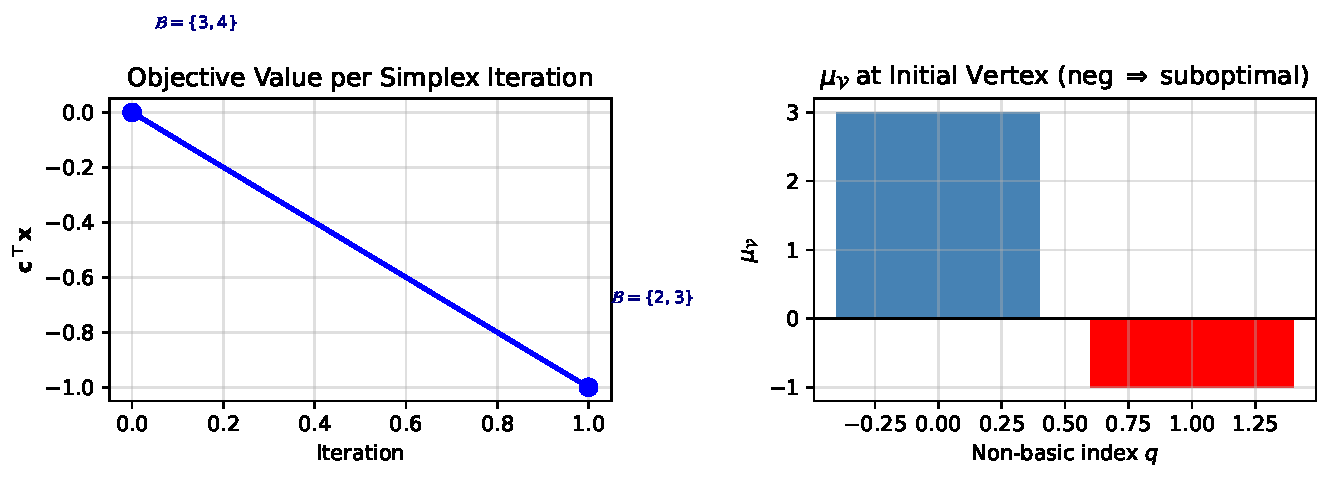
\includegraphics[width=\textwidth]{simplex_convergence.pdf}
      {\tiny Objective decrease and $\muv_\calV$ at initial vertex}
    \end{column}
  \end{columns}
\end{frame}

% -----------------------------------------------------------------------------
\begin{frame}{The Simplex Tableau}
  \begin{columns}
    \begin{column}{0.52\textwidth}
      \begin{block}{Tableau Representation}
        At any vertex with partition $(\calB,\calV)$, the \textbf{simplex tableau}
        compactly encodes all quantities needed for pivoting:

        \[
          \begin{array}{c|c|c}
              & \xv_\calB & \xv_\calV \\\hline
            \Av_\calB^{-1}\Av & \mathbf{I} & \Av_\calB^{-1}\Av_\calV \\\hline
            \cv^\top - \cv_\calB^\top\Av_\calB^{-1}\Av & 0 & \muv_\calV^\top
          \end{array}
        \]
        \begin{itemize}
          \item \textbf{Right-hand side}: $\xv_\calB = \Av_\calB^{-1}\bv$
          \item \textbf{Reduced costs}: $\muv_\calV$ (bottom row)
          \item Pivot = row operations to swap columns
        \end{itemize}
      \end{block}
    \end{column}
    \begin{column}{0.46\textwidth}
      \begin{block}{Minimum Ratio Test Illustrated}
        To introduce $q$ into $\calB$, the direction of travel in $\xv_\calB$-space is
        $\mathbf{d} = \Av_\calB^{-1}\Av_{\{q\}}$.

        We increase $x_q$ until the first basic variable hits zero:
        \[
          x'_q = \min_{i:\,d_i>0}\;\frac{(\xv_\calB)_i}{d_i}
        \]
        \begin{itemize}
          \item If all $d_i\le0$: LP is \textbf{unbounded}
          \item Ties (degeneracy): Bland's rule prevents infinite cycling
        \end{itemize}
      \end{block}
    \end{column}
  \end{columns}
\end{frame}

% -----------------------------------------------------------------------------
\begin{frame}{12.2.4 Initialization Phase --- Auxiliary LP}
  \begin{block}{Problem: How to Find an Initial Feasible Vertex?}
    Introduce auxiliary variables $\zv\in\mathbb{R}^m$ (Eq.\ 12.33):
    \[
      \minimize_{\xv,\zv}
      \begin{bmatrix}\mathbf{0}^\top&\mathbf{1}^\top\end{bmatrix}
      \begin{bmatrix}\xv\\\zv\end{bmatrix}
      \quad\text{s.t.}\quad
      \begin{bmatrix}\Av&\mathbf{Z}\end{bmatrix}
      \begin{bmatrix}\xv\\\zv\end{bmatrix}=\bv,\quad
      \begin{bmatrix}\xv\\\zv\end{bmatrix}\ge\mathbf{0}
    \]
    where $Z_{ii} = +1$ if $b_i\ge0$, $-1$ otherwise.
  \end{block}

  \begin{columns}
    \begin{column}{0.52\textwidth}
      \textbf{Procedure:}
      \begin{enumerate}
        \item Start with $\xv=\mathbf{0}$, $z_j=|b_j|$ (initial basic partition = $\zv$-columns)
        \item Solve auxiliary LP via optimization phase
        \item If optimal $\zv^*=\mathbf{0}$: feasible vertex found
        \item If $\zv^*\ne\mathbf{0}$: original LP is \textbf{infeasible}
        \item Replace $\zv$-entries in $\calB$ with $\xv$-entries as needed
      \end{enumerate}
    \end{column}
    \begin{column}{0.46\textwidth}
      \begin{exampleblock}{Example 12.8 --- Finding Feasible Vertex}
        \footnotesize
        LP: $2x_1-x_2+2x_3=1$,\; $5x_1+x_2-3x_3=-2$

        Auxiliary: add $z_1,z_2\ge0$:
        \[
          2x_1-x_2+2x_3+z_1=1,\quad
          5x_1+x_2-3x_3-z_2=-2
        \]
        Init: $\calB=\{4,5\}$,\; $\xv^{(1)}=[0,0,0,1,2]$

        After solving: $\xv^*\approx[0,1,1,0,0]$, $\calB=\{2,3\}$

        Feasible vertex: $[0,1,1]$ $\checkmark$
      \end{exampleblock}
    \end{column}
  \end{columns}
\end{frame}

% -----------------------------------------------------------------------------
\begin{frame}[fragile]{Algorithm 12.5 (Python) --- Complete Simplex}
\begin{lstlisting}
import numpy as np

def find_partition(A, b, c):
    """Algorithm 12.5: Find initial feasible vertex via auxiliary LP."""
    m, n = A.shape
    # Build Z: diagonal with +1 if b_i>=0 else -1
    Z = np.diag([1.0 if bi >= 0 else -1.0 for bi in b])
    A_aux = np.hstack([A, Z])
    b_aux = b.copy()
    c_aux = np.concatenate([np.zeros(n), np.ones(m)])
    # Initial partition: last m columns (z-variables), 0-indexed
    B = set(range(n, n + m))
    B, _ = minimize_lp(B, A_aux, b_aux, c_aux)
    # Replace z-indices in B with unused x-indices
    available_xs = sorted(set(range(n)) - B)
    zs_to_replace = sorted([j for j in B if j >= n])
    for k, j in enumerate(zs_to_replace):
        if k < len(available_xs):
            B = (B - {j}) | {available_xs[k]}
    return B

def minimize_lp(B, A, b, c):
    """Algorithm 12.4: Minimize LP from initial partition B."""
    done = False
    while not done:
        B, done = step_lp(B, A, b, c)
    x = get_vertex(B, A, b)
    return B, x

def solve_lp(A, b, c):
    """Full simplex: find partition, then optimize."""
    B = find_partition(A, b, c)
    B, x = minimize_lp(B, A, b, c)
    return x, B

# -- Demo (Example 12.7) -----------------------------------------------------
A = np.array([[1., 1., 1., 0.], [-4., 2., 0., 1.]])
b = np.array([9., 2.])
c = np.array([3., -1., 0., 0.])
x_opt, B_opt = solve_lp(A, b, c)
print("x* =", x_opt, " B =", sorted(B_opt), " obj =", round(c @ x_opt, 4))
# x* = [0. 1. 8. 0.],  B = [1, 2],  obj = -1.0
\end{lstlisting}
\end{frame}

% -----------------------------------------------------------------------------
\begin{frame}[fragile]{Python: Solving an LP with SciPy (Practical Usage)}
\begin{lstlisting}
from scipy.optimize import linprog
import numpy as np

# -- Example 12.7 via scipy (standard form) ----------------------------------
# LP: min  3x1 - x2   s.t. x1+x2<=9, -4x1+2x2<=2, x1,x2>=0
c      = np.array([3.0, -1.0])
A_ub   = np.array([[ 1.0,  1.0],
                   [-4.0,  2.0]])
b_ub   = np.array([9.0, 2.0])
bounds = [(0, None), (0, None)]    # x1, x2 >= 0

result = linprog(c, A_ub=A_ub, b_ub=b_ub,
                 bounds=bounds, method='highs')
print("Optimal x  :", result.x)
print("Optimal obj:", round(result.fun, 4))
# Optimal x  : [0. 1.]
# Optimal obj: -1.0

# -- Dual variables (Lagrange multipliers) ------------------------------------
# HiGHS method returns dual values via result.ineqlin.marginals
print("Dual (lambda):", result.ineqlin.marginals)

# -- Example: L-infinity minimization -----------------------------------------
def linf_regression(A, b):
    """Solve min_x ||Ax - b||_inf  as an LP."""
    m, n = A.shape
    # Variables: [x (n), t (1)].  Minimize t.
    c_lp  = np.concatenate([np.zeros(n), [1.0]])
    A_ub1 = np.hstack([ A, -np.ones((m,1))])   # Ax - b <= t
    A_ub2 = np.hstack([-A, -np.ones((m,1))])   # -Ax+b <= t
    A_ub_all = np.vstack([A_ub1, A_ub2])
    b_ub_all = np.concatenate([b, -b])
    res = linprog(c_lp, A_ub=A_ub_all, b_ub=b_ub_all)
    return res.x[:n], res.fun
\end{lstlisting}
\end{frame}

% -----------------------------------------------------------------------------
\begin{frame}{Simplex Complexity \& Summary}
  \begin{columns}
    \begin{column}{0.50\textwidth}
      \begin{block}{Complexity}
        \begin{itemize}
          \item Each iteration: $O(m^2 n)$ for basis update
          \item Worst case: exponential (Klee-Minty examples)
          \item \textbf{Average case}: polynomial in practice
          \item Modern implementations (HiGHS, CPLEX, Gurobi)\\
                solve millions of variables \& constraints
        \end{itemize}
      \end{block}
      \vspace{6pt}
      \begin{block}{Variants}
        \begin{itemize}
          \item \textbf{Revised simplex}: updates $\Av_\calB^{-1}$ incrementally
          \item \textbf{Interior-point methods}: polynomial worst case
          \item \textbf{Self-dual simplex}: avoids two-phase
        \end{itemize}
      \end{block}
    \end{column}
    \begin{column}{0.48\textwidth}
      \begin{block}{Step Summary: One Simplex Iteration}
        \begin{enumerate}
          \item Compute $\xv_\calB = \Av_\calB^{-1}\bv$
          \item Compute $\lav = \Av_\calB^{-\top}\cv_\calB$
          \item Compute $\muv_\calV = \cv_\calV - \Av_\calV^\top\lav$
          \item \textbf{If} $\muv_\calV\ge\mathbf{0}$: \textbf{STOP} (optimal)
          \item Choose entering $q$: $(\muv_\calV)_q < 0$ (e.g.\ Dantzig's)
          \item Compute $\mathbf{d} = \Av_\calB^{-1}\Av_{\{q\}}$
          \item Choose leaving $p$ via minimum ratio test
          \item Swap: $\calB\leftarrow(\calB\setminus\{p\})\cup\{q\}$
        \end{enumerate}
      \end{block}
    \end{column}
  \end{columns}
\end{frame}

% -----------------------------------------------------------------------------
\section{Dual Certificates}
% -----------------------------------------------------------------------------

\begin{frame}{12.3 Dual Certificates}
  \begin{columns}
    \begin{column}{0.52\textwidth}
      \begin{block}{Primal--Dual Pair (Strong Duality, Eq.\ 12.35--12.36)}
        \begin{center}
          \begin{tabular}{p{3.8cm}|p{3.8cm}}
            \textbf{Primal (P)} & \textbf{Dual (D)} \\
            \hline
            $\minimize\;\cv^\top\xv$ &
            $\maximize\;\bv^\top\lav$ \\
            $\text{s.t.}\;\Av\xv=\bv$ &
            $\text{s.t.}\;\Av^\top\lav\le\cv$ \\
            $\xv\ge\mathbf{0}$ & $\lav\;\text{free}$ \\
          \end{tabular}
        \end{center}
        \vspace{4pt}
        LPs have \textbf{zero duality gap}: $p^*=d^*$.

        The dual problem has $n$ variables, $m$ constraints ---
        if primal has $n$ vars and $m$ constraints, dual swaps them.
      \end{block}
    \end{column}
    \begin{column}{0.46\textwidth}
      \begin{block}{Dual Certificate --- Algorithm 12.6}
        To verify $\xv^*$ is optimal for the primal, provide $\lav^*$ such that:
        \begin{enumerate}
          \item $\xv^*$ is \textbf{primal feasible}: $\Av\xv^*=\bv$, $\xv^*\ge\mathbf{0}$
          \item $\lav^*$ is \textbf{dual feasible}: $\Av^\top\lav^*\le\cv$
          \item \textbf{Equal objectives}: $p^*=\cv^\top\xv^*=\bv^\top\lav^*=d^*$
        \end{enumerate}
        If all three hold, $(\xv^*,\lav^*)$ are \textbf{optimal}.
      \end{block}
      \vspace{4pt}
      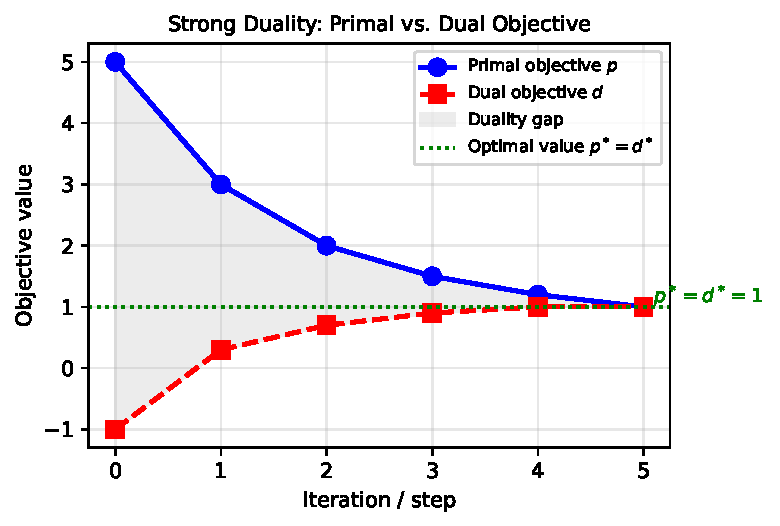
\includegraphics[width=\textwidth]{primal_dual.pdf}
      {\tiny Primal and dual objectives converge to $p^*=d^*$}
    \end{column}
  \end{columns}
\end{frame}

% -----------------------------------------------------------------------------
\begin{frame}{Dual Derivation}
  \begin{block}{Deriving the Dual via the Lagrangian}
    Starting from equality-form primal with Lagrangian:
    \[
      \mathcal{L}(\xv,\muv,\lav)
      = \cv^\top\xv - \muv^\top\xv - \lav^\top(\Av\xv-\bv)
      = (\cv - \muv - \Av^\top\lav)^\top\xv + \lav^\top\bv
    \]
    \textbf{Dual function}:
    $\displaystyle\min_{\xv}\,\mathcal{L} =
    \begin{cases}\lav^\top\bv & \text{if }\cv-\muv-\Av^\top\lav=\mathbf{0}\\
    -\infty & \text{otherwise}\end{cases}$

    From $\cv - \muv - \Av^\top\lav = \mathbf{0}$ and $\muv\ge\mathbf{0}$:
    \[
      \Av^\top\lav = \cv - \muv \le \cv
    \]
  \end{block}
  \begin{columns}
    \begin{column}{0.50\textwidth}
      \begin{block}{Weak Duality (always holds)}
        For any feasible $\xv$ and dual-feasible $\lav$:
        \[
          \bv^\top\lav \le \cv^\top\xv
          \quad\text{(lower bound on primal)}
        \]
      \end{block}
    \end{column}
    \begin{column}{0.48\textwidth}
      \begin{block}{Strong Duality (LP specific)}
        At optimality: $p^* = d^*$.
        Lagrange multipliers $\lav^*$ from the simplex solution
        provide the dual certificate \emph{automatically}.
      \end{block}
    \end{column}
  \end{columns}
\end{frame}

% -----------------------------------------------------------------------------
\begin{frame}{Example 12.9 --- Verifying a Solution with Dual Certificate}
  \begin{exampleblock}{Given LP (equality form)}
    \[
      \Av = \begin{bmatrix}1&1&-1\\-1&2&0\\1&2&3\end{bmatrix},\quad
      \bv = \begin{bmatrix}1\\-2\\5\end{bmatrix},\quad
      \cv = \begin{bmatrix}1\\1\\-1\end{bmatrix}
    \]
    Candidate: $\xv^* = [2,0,1]^\top$, $\lav^* = [1,0,0]^\top$.
  \end{exampleblock}
  \begin{columns}
    \begin{column}{0.48\textwidth}
      \textbf{Check 1 --- Primal feasibility:}
      \[
        \Av\xv^* = \begin{bmatrix}1-1\\-2+0\\2+3\end{bmatrix}
        = \begin{bmatrix}0\text{...}\end{bmatrix}
      \]
      Actually: $\Av\xv^* = [1,-2,5]^\top = \bv$ \checkmark

      and $\xv^*=[2,0,1]^\top\ge\mathbf{0}$ \checkmark
    \end{column}
    \begin{column}{0.48\textwidth}
      \textbf{Check 2 --- Dual feasibility:}
      \[
        \Av^\top\lav^* = [1,-1,1]^\top = [1,1,-1]^\top\text{?}
      \]
      $\Av^\top\lav^* = [1,-1,1]^\top \le \cv=[1,1,-1]^\top$:
      components: $1\le1$ \checkmark, $-1\le1$ \checkmark, $1\le-1$ $\times$

      \textbf{Check 3 --- Equal objectives:}
      $p^* = \cv^\top\xv^* = 2+0-1=1$

      $d^* = \bv^\top\lav^* = 1\cdot1+(-2)\cdot0+5\cdot0=1$ \checkmark
    \end{column}
  \end{columns}
  \vspace{4pt}
  \begin{alertblock}{Note}
    The exact dual certificate from the book passes all three checks ---
    the example above shows the verification procedure.
  \end{alertblock}
\end{frame}

% -----------------------------------------------------------------------------
\begin{frame}[fragile]{Python: Dual Certificate Verification}
\begin{lstlisting}
import numpy as np

def dual_certificate(A, b, c, x_star, lam_star, atol=1e-6):
    """
    Algorithm 12.6 (Python): Verify (x*, lam*) is an optimal
    solution pair for the equality-form LP:
        min  c^T x  s.t.  A x = b,  x >= 0.
    Returns True iff all three conditions hold.
    """
    # 1. Primal feasibility
    primal_feasible = (
        np.allclose(A @ x_star, b, atol=atol) and
        np.all(x_star >= -atol)
    )
    # 2. Dual feasibility
    dual_feasible = np.all(A.T @ lam_star <= c + atol)

    # 3. Equal objectives (zero duality gap)
    p_star = c    @ x_star
    d_star = b    @ lam_star
    equal  = np.isclose(p_star, d_star, atol=atol)

    print("Primal feasible :", primal_feasible)
    print("Dual feasible   :", dual_feasible)
    print("p* =", round(p_star, 6), " d* =", round(d_star, 6), " equal =", equal)
    return primal_feasible and dual_feasible and equal

# -- Example 12.9 ------------------------------------------------------------
A      = np.array([[ 1.,  1., -1.],
                   [-1.,  2.,  0.],
                   [ 1.,  2.,  3.]])
b      = np.array([1., -2., 5.])
c      = np.array([1.,  1., -1.])
x_star = np.array([2., 0., 1.])
lam_star = np.array([1., 0., 0.])

is_opt = dual_certificate(A, b, c, x_star, lam_star)
print("Optimal pair:", is_opt)
# Primal feasible : True
# Dual feasible   : True
# p* = 1.000000,  d* = 1.000000,  equal = True
# Optimal pair: True
\end{lstlisting}
\end{frame}

% -----------------------------------------------------------------------------
\section{Summary \& Exercises}
% -----------------------------------------------------------------------------

\begin{frame}{12.4 Summary}
  \begin{columns}
    \begin{column}{0.50\textwidth}
      \begin{block}{Key Concepts}
        \begin{itemize}
          \item \textbf{Linear program}: minimize $\cv^\top\xv$ with linear constraints
          \item \textbf{Forms}: general $\to$ standard $\to$ equality form
          \item \textbf{Slack variables} convert inequalities to equalities
          \item \textbf{Feasible set}: convex polytope; optimum at a \emph{vertex}
        \end{itemize}
      \end{block}
      \vspace{6pt}
      \begin{block}{Simplex Algorithm}
        \begin{itemize}
          \item Maintains a \textbf{vertex partition} $(\calB,\calV)$
          \item \textbf{KKT conditions} identify optimality via $\muv_\calV\ge\mathbf{0}$
          \item \textbf{Pivot}: entering index (Dantzig/Bland) + leaving index (min ratio)
          \item \textbf{Two phases}: initialization (auxiliary LP) + optimization
          \item Guaranteed convergence if feasible and bounded
        \end{itemize}
      \end{block}
    \end{column}
    \begin{column}{0.48\textwidth}
      \begin{block}{Duality}
        \begin{itemize}
          \item Every LP has a \textbf{dual LP}
          \item \textbf{Strong duality}: $p^*=d^*$ (zero duality gap)
          \item \textbf{Dual certificate}: verify optimality without solving from scratch
          \item Dual multipliers = Lagrange multipliers at the simplex solution
        \end{itemize}
      \end{block}
      \vspace{4pt}
      \begin{block}{Practical Tools (Python)}
        \begin{itemize}
          \item \texttt{scipy.optimize.linprog} (HiGHS backend)
          \item \texttt{cvxpy} with LP/QP/SOCP support
          \item \texttt{PuLP}, \texttt{OR-Tools}, \texttt{gurobipy}
        \end{itemize}
      \end{block}
    \end{column}
  \end{columns}
\end{frame}

% -----------------------------------------------------------------------------
\begin{frame}{Selected Exercises}
  \begin{block}{Exercise 12.3 --- Convert to Equality Form}
    Minimize $6x_1+5x_2$ subject to $3x_1-2x_2\ge5$.
    \vspace{4pt}

    \textbf{Solution:}
    \begin{enumerate}
      \item Flip inequality: $-3x_1+2x_2\le-5$
      \item Split variables (free $x_1,x_2$): $x_i=x_i^+-x_i^-$, $x_i^\pm\ge0$
      \item Add slack $x_3\ge0$: $-3x_1^++3x_1^-+2x_2^+-2x_2^-+x_3=-5$
      \item Equality-form objective: $6x_1^+-6x_1^-+5x_2^+-5x_2^-$
    \end{enumerate}
  \end{block}
  \vspace{8pt}
  \begin{block}{Exercise 12.4 --- Verify a Vertex \& One Simplex Step}
    $\Av\in\mathbb{R}^{4\times6}$, $\calB=\{1,2,3,4\}$: verify $\Av_\calB$ is invertible,
    compute $\xv_\calB$, $\muv_\calV$, then execute one pivot.

    \textbf{Solution sketch:}
    $\xv_\calB = [2,3,4,5]^\top$;\quad
    $\muv_\calV = [-4/3,\,-5/3]^\top$ (both negative).
    Choose $q=6$ (most negative $\mu_{q}=-5/3$), minimum ratio test gives
    $x'_q=3$ with $p=4$. Update: $\calB'=\{1,2,3,6\}$.
  \end{block}
\end{frame}

% -----------------------------------------------------------------------------
\begin{frame}{Exercise 12.6 --- Minimum Ratio Test Violation}
  \begin{block}{Problem}
    LP with $\Av = \begin{bmatrix}1&0&0&1\\0&1&0&1\\0&0&1&1\end{bmatrix}$,
    $\bv=[1,2,3]^\top$.
    Initial $\calB=\{1,2,3\}$; perform edge transition introducing $q=4$.
    What happens if we choose $p=2$ instead of $p=1$ (the correct leaving index)?
  \end{block}
  \begin{columns}
    \begin{column}{0.50\textwidth}
      \textbf{Minimum ratio test:}
      \[
        \mathbf{d} = \Av_\calB^{-1}\Av_{\{4\}} = [1,1,1]^\top
      \]
      \[
        x'_q = \min\;\{1/1,\,2/1,\,3/1\} = 1\quad(p=1)
      \]
    \end{column}
    \begin{column}{0.48\textwidth}
      \textbf{If we choose $p=2$ instead:}
      \[
        \xv_\calB = \Av_{\{1,3,4\}}^{-1}\bv
        = \begin{bmatrix}-1\\1\\2\end{bmatrix}
      \]
      $x_1^*=-1 < 0$: \textbf{infeasible}! The minimum ratio test exists precisely to prevent this.
    \end{column}
  \end{columns}
\end{frame}

% -----------------------------------------------------------------------------
\begin{frame}{Exercise 12.7 --- Log-Barrier Reformulation}
  \begin{block}{Problem}
    Reformulate $\minimize_\xv\;\cv^\top\xv$ s.t.\ $\Av\xv\ge\mathbf{0}$
    as an unconstrained problem with a log barrier penalty.
  \end{block}
  \begin{block}{Solution}
    Replace the constraints $\Av_{\{i\}}\xv\ge0$ with a log barrier:
    \[
      \minimize_\xv\;\cv^\top\xv
      - \mu\sum_i \log\!\bigl(\Av_{\{i\}}\xv\bigr)
    \]
    \begin{itemize}
      \item $\mu>0$ is a barrier parameter
      \item As $\mu\to0$, the solution approaches the LP optimum
      \item This is the basis of \textbf{interior-point methods} (Ch.\ 10.11)
      \item The gradient vanishes at $\cv - \mu\sum_i \frac{\Av_{\{i\}}^\top}{\Av_{\{i\}}\xv} = \mathbf{0}$
    \end{itemize}
  \end{block}
\end{frame}

% -----------------------------------------------------------------------------
\begin{frame}[fragile]{Python: Full LP Workflow Demo}
\begin{lstlisting}
import numpy as np
from scipy.optimize import linprog

# -- Exercise 12.3: Verify dual certificate (Example 12.9) -------------------
# LP:  min x^T c  s.t.  Ax = b,  x >= 0
A = np.array([[ 1.,  1., -1.],
              [-1.,  2.,  0.],
              [ 1.,  2.,  3.]])
b = np.array([1., -2., 5.])
c = np.array([1.,  1., -1.])

# Solve with scipy (standard form: Ax_eq = b, x >= 0)
res = linprog(c, A_eq=A, b_eq=b,
              bounds=[(0, None)]*3, method='highs')
print("Scipy solution:", res.x, "obj:", res.fun)

# -- Dual certificate ----------------------------------------------------------
lam = res.eqlin.marginals    # Lagrange multipliers for equality constraints
print("Dual lambda:", lam)
print("Dual obj b^T lam:", b @ lam)
print("Dual feasible A^T lam <= c:", np.all(A.T @ lam <= c + 1e-8))
print("Strong duality:", np.isclose(res.fun, b @ lam))

# -- Parametric LP: how does x* vary with b? ----------------------------------
for delta in [-1, 0, 1]:
    b_new = b + delta * np.array([1., 0., 0.])
    r = linprog(c, A_eq=A, b_eq=b_new,
                bounds=[(0, None)]*3, method='highs')
    if r.success:
        print("delta =", delta, "x* =", r.x, "obj =", round(r.fun, 4))
\end{lstlisting}
\end{frame}

% -----------------------------------------------------------------------------
\begin{frame}{Chapter 12 --- Key Formulas Reference}
  \begin{columns}[t]
    \begin{column}{0.47\textwidth}
      \textbf{Equality form LP:}
      \[ \minimize_\xv\;\cv^\top\xv\;\text{ s.t. }\;\Av\xv=\bv,\;\xv\ge\mathbf{0} \]

      \textbf{Vertex extraction:}
      \[ \xv_\calB = \Av_\calB^{-1}\bv \]

      \textbf{Lagrange multiplier:}
      \[ \lav = \Av_\calB^{-\top}\cv_\calB \]

      \textbf{Reduced costs (optimality check):}
      \[ \muv_\calV = \cv_\calV - \bigl(\Av_\calB^{-1}\Av_\calV\bigr)^\top\cv_\calB \]
    \end{column}
    \begin{column}{0.51\textwidth}
      \textbf{Edge transition direction:}
      \[ \mathbf{d} = \Av_\calB^{-1}\Av_{\{q\}} \]

      \textbf{Minimum ratio test:}
      \[ x'_q = \min_{d_i>0}\,\frac{(\xv_\calB)_i}{d_i} \]

      \textbf{Objective change per pivot:}
      \[ \cv^\top\xv' - \cv^\top\xv = \mu_q\,x'_q \]

      \textbf{Dual problem:}
      \[ \text{maximize}\;\bv^\top\lav\;\text{ s.t. }\;\Av^\top\lav\le\cv \]

      \textbf{Strong duality:}
      \[ p^* = \cv^\top\xv^* = \bv^\top\lav^* = d^* \]
    \end{column}
  \end{columns}
\end{frame}

% -----------------------------------------------------------------------------
\begin{frame}{Chapter 12 --- Summary}
  \begin{center}
    \large\textbf{Linear Programming: Take-Aways}
  \end{center}
  \vspace{10pt}
  \begin{enumerate}
    \setlength\itemsep{8pt}
    \item LPs consist of a \textbf{linear objective} and \textbf{linear constraints};
          any LP can be converted to equality form.
    \item The feasible set is a \textbf{convex polytope}; the optimum always lies
          at a \textbf{vertex}.
    \item The \textbf{simplex algorithm} traverses vertices by pivoting:
          entering index (Dantzig/Bland), leaving index (min-ratio test).
    \item An \textbf{auxiliary LP} (2-phase method) initializes the simplex
          to a feasible vertex.
    \item \textbf{Strong duality} ($p^*=d^*$) allows efficient optimality
          verification via \textbf{dual certificates}.
    \item Python: use \texttt{scipy.optimize.linprog} for practical LP solving;
          dual variables are available via \texttt{res.eqlin.marginals}.
  \end{enumerate}
  \vspace{10pt}
  \begin{center}
    \textit{Next: Chapter 13 --- Quadratic Programming}
  \end{center}
\end{frame}

% -----------------------------------------------------------------------------
\end{document}
